\documentclass[
	fontsize=12pt,          % default font size 12pt
	paper=a4,               % DIN A4 page format
	numbers=noenddot,       % remove dots behind chapter numbers (e.g. 1.5 not 1.5.)
	listof=totoc,           % add list of figures, tables, etc. to ToC
	listof=entryprefix,     % add entry name to figures, tables, etc.
	listof=nochaptergap,    % no chapter gap for figures, tables, etc.
	bibliography=totoc,     % add bibliography to ToC but without a chapter number
	parskip=half,           % half line spacing between paragraphs
	openany                 % chapters can start on any page
]{scrbook}

\include{../../for_latex/preamble}

\usepackage{tikz}
\usetikzlibrary{trees,calc}

\begin{document}

\begin{titlepage}
	\pagestyle{empty}

	% HFU Logo
	\begin{flushright}
		\begin{figure}[ht]
			\flushright
			
\includegraphics[height=2cm]{../../for_latex/hfu}
		\end{figure}
	\end{flushright}

	\begin{center}
		\vspace{3cm}

		{\fontsize{22}{22} \selectfont \textbf{Blatt 1}}\\[5mm]
		{\fontsize{18}{18} \selectfont Grundlagen der IT-Sicherheit}

		\vspace{12cm}

		{\fontsize{14}{14} \selectfont Luis Staudt}
	\end{center}
\end{titlepage}

% ############################################################################
% CONTENT STARTS HERE
% ############################################################################

\chapter*{Aufgabe 1: Die drei Schutzziele}

\section*{Vertraulichkeit (Confidentiality)}
Vertraulichkeit bedeutet, dass Informationen nur von autorisierten Personen eingesehen werden können.
Unbefugte Dritte dürfen keinen Zugang zu geschützten Daten erhalten.
Die Einhaltung ist wichtig, weil ein Verstoß zu Datenlecks, Identitätsdiebstahl oder Wirtschaftsspionage führen kann.
Beispiele für Maßnahmen sind Verschlüsselung, Zugriffskontrollen und Need-to-know-Prinzipien.

\section*{Integrität (Integrity)}
Integrität stellt sicher, dass Daten vollständig und unverändert bleiben.
Änderungen dürfen nur durch berechtigte Personen in nachvollziehbarer Weise erfolgen.
Die Einhaltung ist wichtig, weil manipulierte Daten zu falschen Entscheidungen, fehlerhaften Transaktionen oder dem Verlust von Vertrauen führen können.
Maßnahmen wie Hashwerte, digitale Signaturen und Versionierung schützen die Integrität.

\section*{Verfügbarkeit (Availability)}
Verfügbarkeit bedeutet, dass Systeme und Daten für berechtigte Nutzer jederzeit innerhalb eines vereinbarten Zeitrahmens zugänglich sind.
Die Einhaltung ist wichtig, weil Ausfälle zu finanziellen Verlusten, Produktionsstillstand oder sogar Gefahr für Menschenleben (z.\,B. in der Medizintechnik) führen können.
Redundanz, Backups und Notfallpläne sind typische Schutzmaßnahmen.


\chapter*{Aufgabe 2: Gefahren für die Schutzziele}

\begin{tabularx}{\textwidth}{@{} l X X @{}}
	\toprule
	Gefahr & Beschreibung & Bedrohtes Schutzziel \\
	\midrule
	Phishing-Angriff &
	Ein Angreifer versendet gefälschte E-Mails, die Nutzer dazu verleiten, ihre Zugangsdaten auf einer nachgebauten Website einzugeben.
	Der Angreifer erhält so Zugriff auf vertrauliche Informationen. &
	Vertraulichkeit: Unbefugte erhalten Zugang zu geschützten Daten. \\[6pt]

	Ransomware &
	Schadsoftware verschlüsselt die Dateien eines Opfers und fordert ein Lösegeld für die Entschlüsselung.
	Häufig werden dabei auch Daten manipuliert oder gelöscht. &
	Integrität und Verfügbarkeit: Daten werden verändert und sind nicht mehr zugänglich. \\[6pt]

	DDoS-Angriff &
	Ein verteilter Denial-of-Service-Angriff überflutet einen Server mit so vielen Anfragen, dass dieser überlastet wird und für legitime Nutzer nicht mehr erreichbar ist. &
	Verfügbarkeit: Der Dienst steht autorisierten Nutzern nicht mehr zur Verfügung. \\
	\bottomrule
\end{tabularx}


\chapter*{Aufgabe 3: Szenario E-Mail im Urlaub}

\section*{a) Was ist geschehen?}
Alice (die Urlauberin) hat Bob (die bekannte Person) per E-Mail gebeten, ihre Blumen zu gießen, und dabei ihre Adresse sowie den Aufbewahrungsort des Haustürschlüssels mitgeteilt.
Eve (die Angreiferin) hat diese E-Mail abgefangen und mitgelesen.
Mit den gewonnenen Informationen (Adresse, Schlüsselversteck und Wissen über Alices Abwesenheit) konnte Eve die Wohnung betreten und die Einrichtung stehlen.
Bob hat die E-Mail möglicherweise nie erhalten oder den Inhalt nicht gelesen, weshalb die Blumen nicht gegossen wurden.

\section*{b) Verletztes Schutzziel}
Es wurde das Schutzziel der Vertraulichkeit verletzt.
Die E-Mail mit den sensiblen Informationen (Adresse, Schlüsselversteck, Abwesenheitszeitraum) wurde von einem unbefugten Dritten mitgelesen.

\section*{c) STRIDE-Bedrohung}
Aus dem STRIDE-Bedrohungsmodell ist Information Disclosure (Verletzung der Vertraulichkeit) eingetroffen.
Vertrauliche Informationen wurden einer nicht autorisierten Partei offengelegt.
Zusätzlich könnte Spoofing eine Rolle spielen, falls Eve die Identität von Bob vorgetäuscht hat.

\newpage
\section*{d) Wie konnte der Angreifer an die E-Mail gelangen?}
Es gibt mehrere mögliche Angriffsvektoren:
\begin{itemize}
	\item Man-in-the-Middle-Angriff: Eve hat den Netzwerkverkehr in einem ungesicherten WLAN (z.\,B. am Flughafen) abgefangen und die unverschlüsselte E-Mail mitgelesen.
	\item Kompromittiertes E-Mail-Konto: Eve hat sich Zugang zum E-Mail-Konto von Alice oder Bob verschafft, z.\,B. durch ein schwaches Passwort oder Credential Stuffing.
	\item Kompromittierter E-Mail-Server: Der E-Mail-Server wurde gehackt, sodass Eve alle übertragenen E-Mails lesen konnte.
	\item Sniffing: Wenn die Übertragung nicht TLS-verschlüsselt war, konnte Eve den Netzwerkverkehr im selben Netzwerk mitlesen.
\end{itemize}

\section*{e) Wie hätte sich das Szenario verhindern lassen?}
\begin{itemize}
	\item Ende-zu-Ende-Verschlüsselung: Nutzung von PGP oder S/MIME, sodass nur Bob die E-Mail entschlüsseln kann.
	\item Alternativer Kommunikationskanal: Sensible Informationen wie das Schlüsselversteck telefonisch oder persönlich übermitteln, nicht per E-Mail.
	\item Sichere Schlüsselübergabe: Ein Schlüsselsafe mit Code verwenden und den Code über einen separaten Kanal mitteilen.
	\item Starke Passwörter und 2FA: Sichere Passwörter und Zwei-Faktor-Authentifizierung für E-Mail-Konten verwenden, um eine Kompromittierung des Kontos zu verhindern.
\end{itemize}


\chapter*{Aufgabe 4: Responsible Disclosure}

\section*{a) Warum ist die Veröffentlichung eine kritische Phase?}
Zwischen Bekanntwerden einer Schwachstelle und der Verfügbarkeit eines Patches besteht ein kritisches Zeitfenster (Window of Vulnerability), in dem Angreifer die Lücke ausnutzen können.
Coordinated Disclosure minimiert dieses Risiko, indem der Finder die Schwachstelle zunächst vertraulich an den Hersteller meldet und eine Frist zur Behebung einräumt (typischerweise 90 Tage), bevor Details veröffentlicht werden.

\section*{b) Full Disclosure und Gegenmaßnahmen}
Full Disclosure bedeutet, dass eine Schwachstelle mit allen technischen Details sofort öffentlich gemacht wird, ohne dem Hersteller vorab Zeit zur Behebung zu geben.
Dies birgt das Risiko eines Zero-Day-Exploits.

Softwareentwickler können Full Disclosure verhindern durch:
\begin{itemize}
	\item Bug-Bounty-Programme als Anreiz für verantwortungsvolle Meldungen.
	\item Klare Meldewege, z.\,B. eine security.txt-Datei oder ein Responsible-Disclosure-Programm.
	\item Schnelle Reaktionszeiten bei gemeldeten Schwachstellen, da Ignorieren die Wahrscheinlichkeit eines Full Disclosure erhöht.
	\item Transparente Kommunikation über den Fortschritt der Behebung.
\end{itemize}


\chapter*{Bonusaufgabe: Attack-Tree}

Der folgende Attack-Tree modelliert die möglichen Angriffspfade aus dem Szenario in Aufgabe 3a.
Das Wurzelziel ist der Einbruch in Alices Wohnung.

\begin{center}
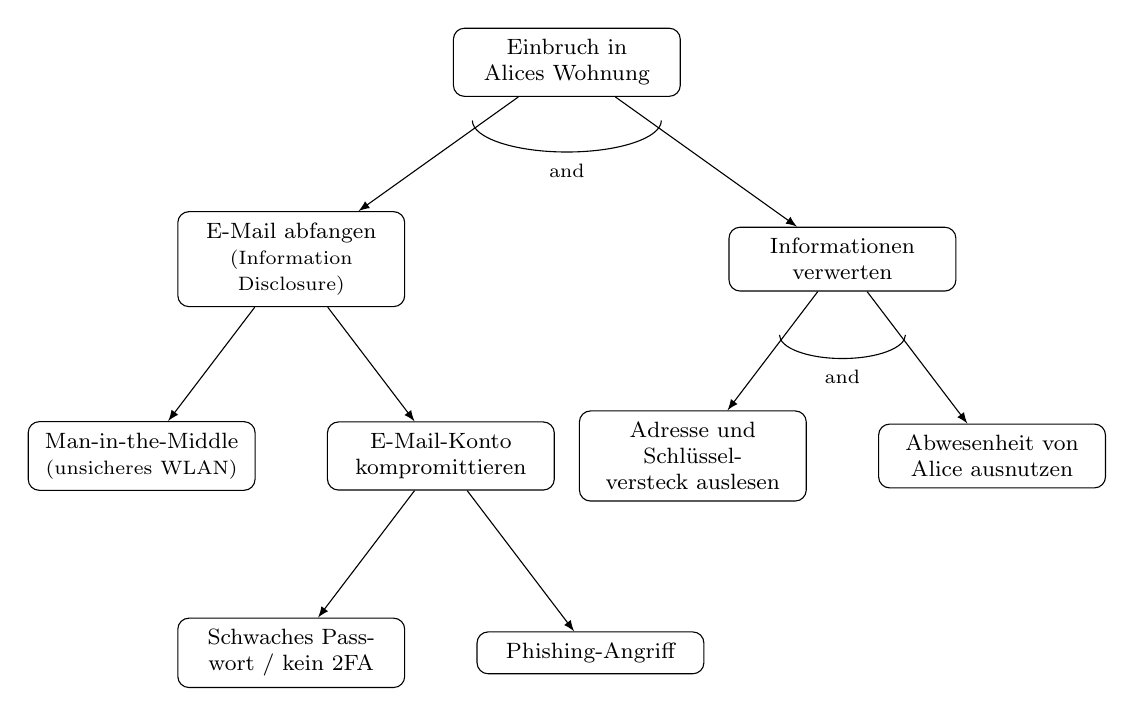
\begin{tikzpicture}[
	grow=down,
	level distance=2.5cm,
	every node/.style={
		draw,
		rounded corners,
		text width=2.6cm,
		align=center,
		font=\footnotesize,
		inner sep=4pt
	},
	edge from parent/.style={draw, -latex},
	level 1/.style={sibling distance=7cm},
	level 2/.style={sibling distance=3.8cm},
	level 3/.style={sibling distance=3.8cm}
]
\node (root) {Einbruch in Alices Wohnung}
	child { node (abfangen) {E-Mail abfangen\\ \scriptsize(Information Disclosure)}
		child { node {Man-in-the-Middle\\ \scriptsize(unsicheres WLAN)} }
		child { node {E-Mail-Konto kompromittieren}
			child { node {Schwaches Passwort / kein 2FA} }
			child { node {Phishing-Angriff} }
		}
	}
	child { node (verwerten) {Informationen verwerten}
		child { node (adresse) {Adresse und Schlüssel\-versteck auslesen} }
		child { node (abwesend) {Abwesenheit von Alice ausnutzen} }
	};

\draw ($(root.south) + (-1.2,-0.3)$) arc[start angle=180, end angle=360, x radius=1.2cm, y radius=0.4cm] node[midway, below, font=\scriptsize, draw=none, text width=0.6cm] {and};

\draw ($(verwerten.south) + (-0.8,-0.55)$) arc[start angle=180, end angle=360, x radius=0.8cm, y radius=0.3cm] node[midway, below, font=\scriptsize, draw=none, text width=0.6cm] {and};
\end{tikzpicture}
\end{center}

Der Attack-Tree zeigt, dass der Angriff aus zwei Hauptphasen besteht:
Zuerst muss Eve an die E-Mail gelangen (linker Teilbaum), dann muss sie die gewonnenen Informationen verwerten (rechter Teilbaum).
Beide Phasen müssen erfolgreich sein (AND-Verknüpfung), damit der Einbruch gelingt.
Äste ohne Bogen sind OR-verknüpft, d.\,h. es genügt, wenn einer der Angriffsvektoren erfolgreich ist.


% ############################################################################
% CONTENT ENDS HERE
% ############################################################################

\end{document}
